%\documentclass[toc]{Template/PoS}
\documentclass{Template/PoS}

\usepackage{enumitem}
\usepackage{soul}
\setlist{nolistsep}

\title{Integrating Network-Awareness and Network-Management into PhEDEx}

\ShortTitle{Network-Management in PhEDEx}

\author{\speaker{Vlad L\v{a}p\v{a}d\v{a}tescu}\\
Caltech / USA\\
E-mail: \email{vlad@cern.ch}}

\author{Tony Wildish\\
Princeton / USA\\
E-mail: \email{awildish@princeton.edu}}

\author{ANSE Collaboration 
	\thanks{B. Ball, A. Barczyk, J. Batista, K. De, S. McKee, A. Melo, H. Newman, A. Petrosyan, P. Sheldon, R. Voicu}}

\abstract{
ANSE (Advanced Network Services for Experiments) is an NSF funded project, which aims
 to incorporate advanced network-aware tools in the mainstream production workflows of 
 LHC's two largest experiments: ATLAS and CMS. For CMS, this translates in the integration 
 of bandwidth provisioning capabilities in PhEDEx, its data-transfer management tool.

PhEDEx controls the large-scale data-flows on the WAN across the experiment, typically
 handling 1 PB of data per week, spread over 70 sites. This is only set to increase 
 once LHC resumes operations in 2015.

The goal of ANSE is to improve the overall working efficiency of the experiments, by 
allowing for more deterministic times to completion for a designated set of data transfers,
 through the use of end-to-end dynamic virtual circuits with guaranteed bandwidth.

Through our work in ANSE, we have enhanced PhEDEx, allowing it to control a circuit's 
lifecycle based on its own needs. By checking its current workload and past transfer 
history on normal links, PhEDEx is now able to make smart use of dynamic circuits, 
only creating one when it's worth doing so. Different circuit management infrastructures
 can be used, via a plug-in system, making it highly adaptable.

In this paper, we present the progress made by ANSE with regards to PhEDEx. We show how
 our system has evolved since our prototype phase we presented last year, and how it is
 now able to make use of dynamic circuits as a production-quality service. We describe 
 its updated software architecture and how this mechanism can be refactored and used 
 as a stand-alone system in other software domains (like ATLAS' PanDA). 

We conclude, by describing the remaining work to be done ANSE (for PhEDEx) and discuss 
on future directions for continued development.
}

\FullConference{International Symposium on Grids and Clouds (ISGC) 2015,\\
		15-20 March 2015\\
		Academia Sinica, Taipei, Taiwan}

\parindent=0pt 

\begin{document}
    
\section{Introduction}
\subsection{PhEDEx}
\subsection{Dynamic circuits}
\subsection{Motivation}
\section{Initial prototype}

\subsection{Introducing circuit awareness}

As described, PhEDEx consists of two different types of agents: 
central and site agents. As such, the integration of dynamic circuits can 
be done at one of those levels.

Even though at a site level only a local, site centric, view of
the network (and transfer queues) exists, it was decided that integrating 
circuit awareness here, was a good compromise between ideal required 
functionality and the complexity of the task at hand.

The initial efforts\cite{ANSE-ISGC} focused on providing a prototype based on the FileDownload
site agent. In addition, for the purposes of this prototype, FDT\cite{FDT} was chosen
as the transfer backend. The FDT tool is a fast, lightweight transfer tool,
which integrates IDCP\footnote{InterDomain Controller Protocol} \cite{IDCP}
OSCARS\cite{OSCARS} (On-Demand Secure Circuits and Advance Reservation System) calls.

\subsection{Standard FileDownload agent}

The FileDownload agent in PhEDEx is one of the site agents\footnote{
Each site runs one or more copies of this agent.} and it's responsible for the
execution of file transfers. The agent (as all PhEDEx agents) is event driven 
using the Perl Object Environment framework, operates in pull mode\footnote{Files are
downloaded from a source site.} and executes transfers from its transfer queue.
The transfer queue is continuously updated by the FileRouter agent and contains 
information about all due transfers from the different source nodes (site) that the agent 
has to execute. For each source-destination pair of PhEDEx nodes, the FileDownload 
agent organizes the files in a way that is suitable for the transfer tool which is 
going to be used. This consists in splitting the queue of files into separate 
transfer jobs. Each transfer jobs usually contains several tens of files.
The agent executes one or more transfer jobs in parallel, depending 
on the site's configuration, then verifies that the files have been correctly 
delivered before reporting back to the database with the transfer results.

At any given time, PhEDEx only knows if two sites have or haven't got connectivity
between them, but knows nothing about the physical network path existing between
them. This means that when dealing with any pair of source-destination nodes, 
the FileDownload agent executes the transfer on the default network path available 
between the two storage servers involved in the transfer. Even if available, the agent
 can't use alternative transfer paths since it has no knowledge of them.

\subsubsection{PFNs and LFNs}

PhEDEx transfers files in bulk, in what is called a transfer job. Each transfer job
knows the source and destination URLs of the file being transferred as well as 
monitoring and logging information. In PhEDEx these URLs are called Physical
File Names (PFNs) and encode the transfer protocol being used, the hostname (or IP)
of the storage on which the file is located and the local path of the file
on the storage. 
The hostname present in the PFN, doesn't necessarily point to the
actual server on which file replicas reside, but points to the entity that knows where 
the file is located. This is particularly important when dealing with FTS\cite{FTS} 
and gridFTP.
The PFNs are actually constructed from Logical File Names (LFNs) and a look-up table
which each site maintains and uploads to the central database.

\subsection{Prototype FileDownload agent}

Since the FileDownload agent is instrumental in transferring files between sites, it was 
picked as the best place where the functionality needed for circuit awareness could be added.

\begin{itemize}
	\item The FileDownload agent, can now estimate the amount of work remaining 
	to be done for each source-destination pair. This estimation is based on simple 
	monitoring statistics that PhEDEx gathers, and information on its own download 
	queue. If there is significant\footnote{arbitrary limit set initially to 6 hours} 
	work remaining to be done, a circuit is requested.
	\item After a circuit is requested, the agent checks for duplicate circuits, creates 
	a status file (used in case of an abnormal agent shutdown), calls the circuit 
	backend for requesting a circuit, then creates a timeout timer for the reply.
	If it doesn't receive a reply from the circuit backend in the allotted time, the 
	request is considered as failed.
	\item Once the reply from the circuit backend is received, the state of the 
	request is updated and saved to disk. A new timer used to teardown the circuit is started.
	\item The FileDowload agent also routinely verifies that the state of circuits 
	in memory matches what was saved on disk.
\end{itemize}

\subsection{Test setup}

The prototype was tested on ANSE's testbed using two PhEDEx test sites (Figure \ref{fig:ANSE-setup}).
Each test site was composed of a storage server and a PhEDEx site server. On each storage
server we used one disk controller managing 8 SSDs. Two 10Gbps virtual circuits were created 
for the purposes of this test. One of the circuits was used to model a shared link in 
which PhEDEx had to compete with other traffic. This background traffic was generated 
by Iperf and consisted of a continuous stream of UDP packets at 5Gbps. The second circuit 
served as the dedicated link. The main purpose of this test wasn't to show that we can 
saturate a 10Gbps link with PhEDEX, but that a PhEDEx FileDownload agent is able to switch 
to using a new path in a transparent manner and with no down time. The first part of 
the test consisted of a 10 hour run with PhEDEx transfers on the shared link. After this 
time, PhEDEx switched to using the dedicated circuit and continued transfers for another 10 
hours. PhEDEx was setup up to run a single 450 GB transfer job at a time, each one 
comprised of 30 files of 15 GB each.

\begin{figure}[h]
  \centering
  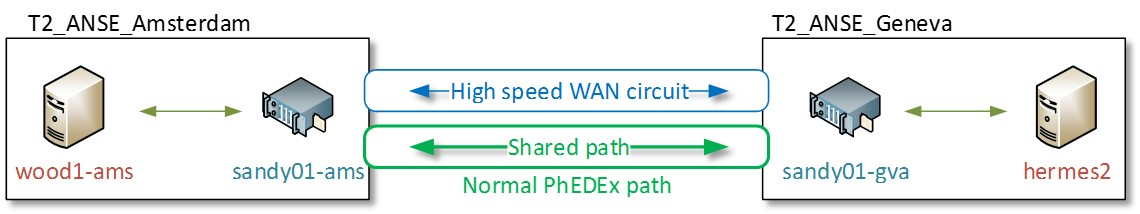
\includegraphics[width=0.95\textwidth]{Figures/FileDownload_ANSE_Testbed.jpg}
  \caption{PhEDEx testbed for ANSE}
  \label{fig:ANSE-setup}
\end{figure}

\subsection{Results}

The results are summarised in Figure \ref{fig:combined_transfers}. This plot portrays the transfer 
speeds that PhEDEx achieved in our test scenario. The left half of the plot shows the PhEDEx 
throughput in the first part of the test while it was competing with the iperf traffic. Naturally, 
this limits PhEDEx traffic to ~600MB/sec (~4800 Gbps). The right part of the plot, displays the 
transfer speeds PhEDEx achieved on an empty link, with no competing traffic. An effective doubling 
of throughput is seen, with PhEDEx being able to fill up the whole 10 Gbps link.
The seesaw look of this plot is linked to the fact that PhEDEx has a delay between finishing one job and 
starting the next. This is due to various factors: pre/post validation, preparation of copyjobs or 
even time spent by the backend itself before actually launching a transfer. Because of these delays, 
the average rates reported by PhEDEx (Figure \ref{fig:combined_phedex_transfers}) will always be lower 
than the average rates of each individual transfer job. 
Lastly, Figure \ref{fig:combined_transfers} also shows the fact that there was no interruption in service 
when PhEDEx moved from one link to another. This test demonstrates the potential usefulness of 
using virtual circuits in PhEDEx.

\begin{figure}[h]
  \centering
  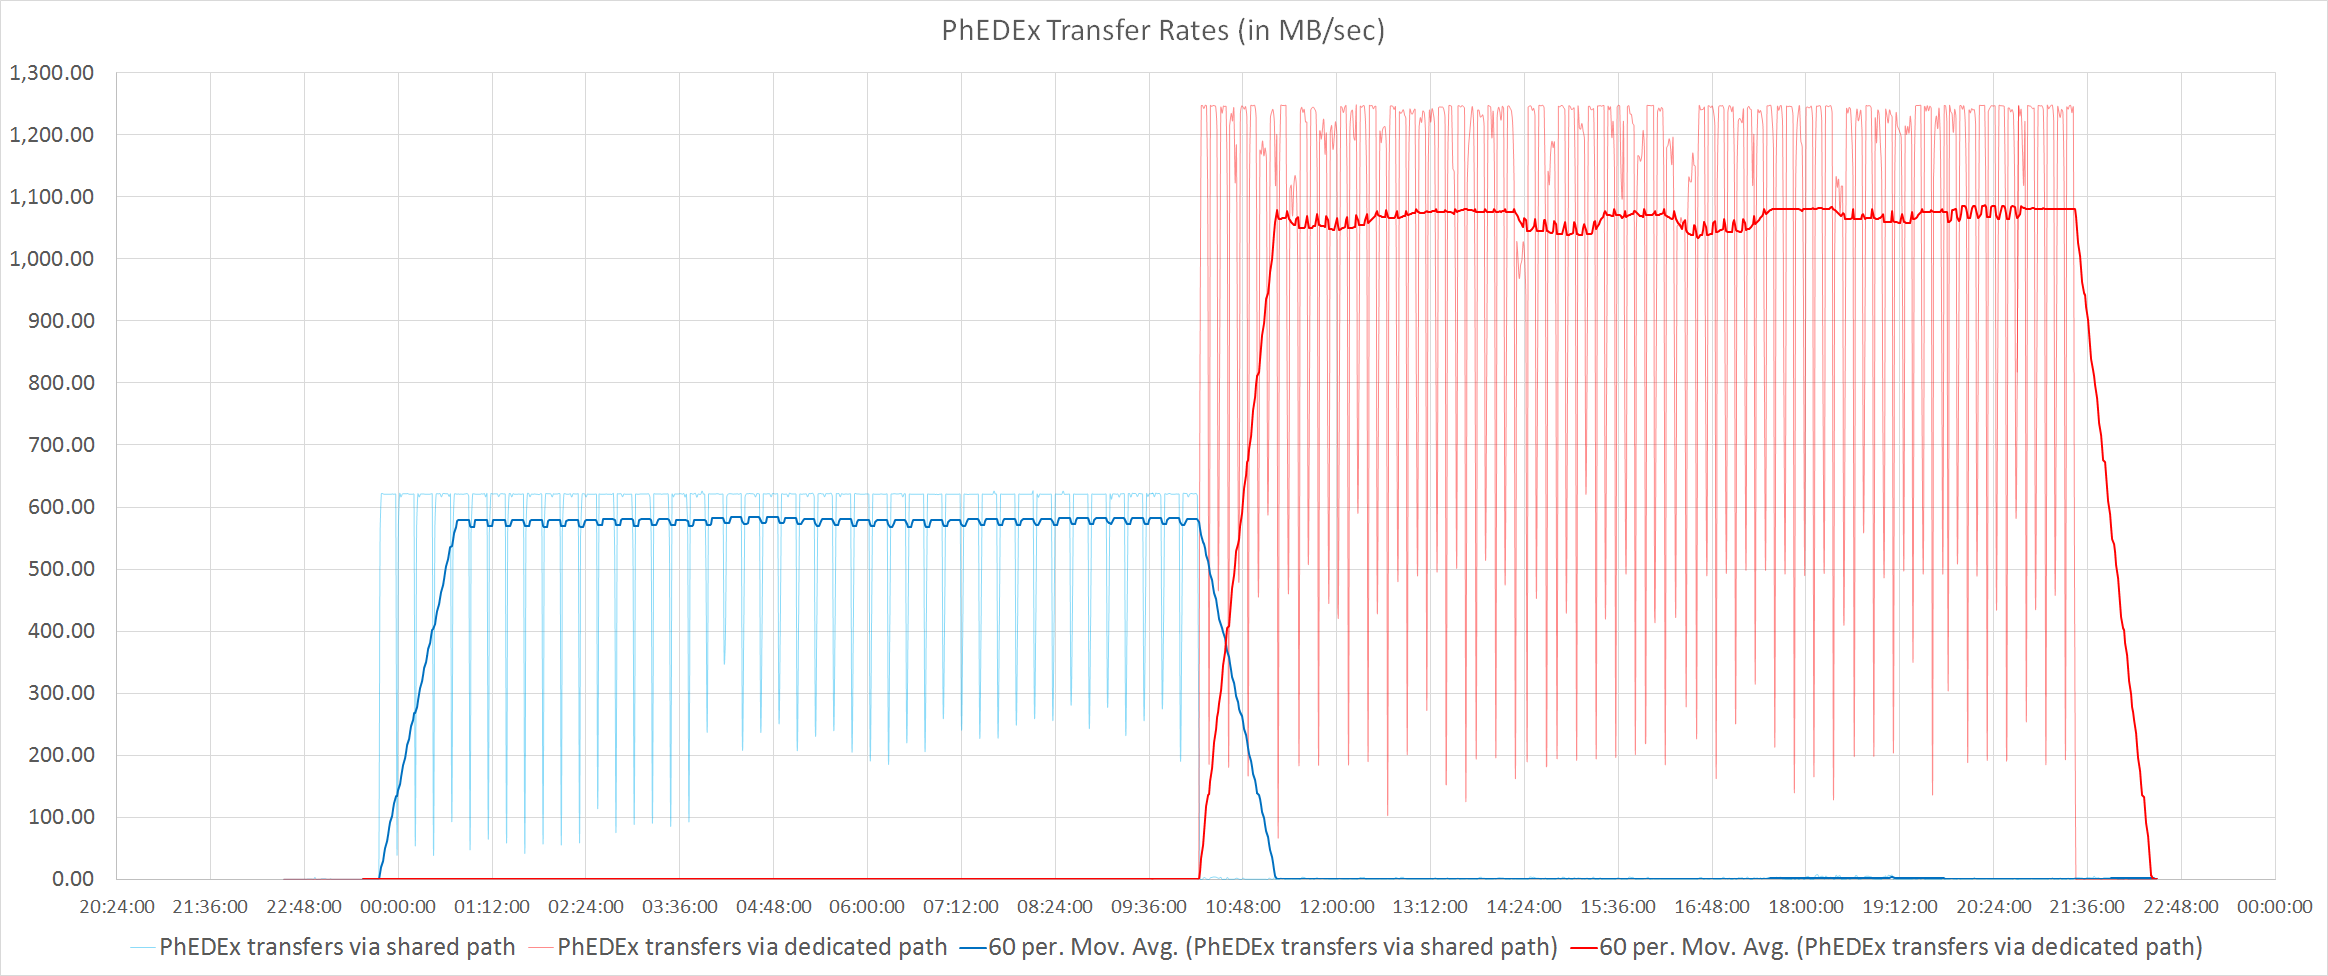
\includegraphics[width=0.95\textwidth]{Figures/FileDownload_All_paths.png}
  \caption{View of PhEDEx-only transfers on both the shared and dedicated path}
  \label{fig:combined_transfers}
\end{figure} 

\begin{figure}[h]
  \centering
  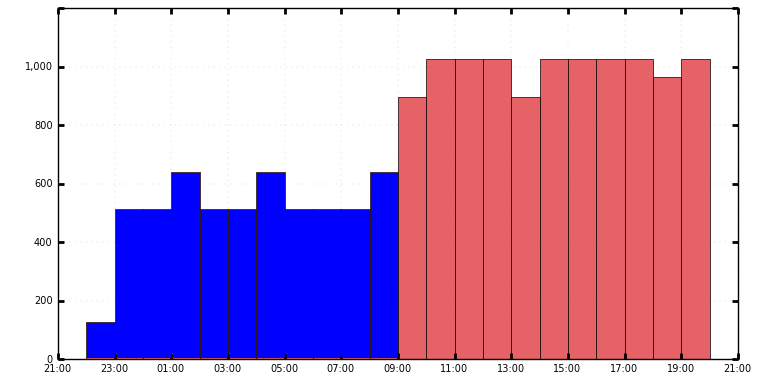
\includegraphics[width=0.95\textwidth]{Figures/FileDownload_PhEDEx_all_paths.png}
  \caption{View of PhEDEx only transfers on both the shared and dedicated path}
  \label{fig:combined_phedex_transfers}
\end{figure} 

\subsection{Prototype limitations}

The prototype proved helpful in demonstrating that circuits can be useful, and that circuit 
awareness can be integrated into PhEDEx, specifically at the site level. The design decisions 
taken in the development process mirror the need for a fast working prototype and this 
ultimately had an impact on its ultimate usefulness.

\begin{itemize}
  \item Non-modular design: All of the control logic was contained in the FileDownload agent.
  This meant that the part that requests circuits and manages their lifecycle could not be 
  separated from the FileDownload agent. This was needed in order to create a stand alone 
  application that could be used external tools as well.
  \item Single circuit backend: Relied on a single method of requesting circuits (DYNES\cite{DYNES}). 
  For every different circuit provider used, a major change in code was required.
  \item Relied on FDT as a transfer tool: Unfortunately, this transfer tool is not widely used
  in production. Our production ready version should at least support the most common protocols
  out there (ie. FTS/SRM/gridFTP)
\end{itemize}

In addition to these decisions, it was assumed that a simple storage system would be used.
In all transfers involving the prototype, data was always moved from server to server, not 
from a storage farm to a storage farm. This becomes an issue when when extrapolating from a 
prototype to a production infrastructure since, it is assumed that the PFNs that PhEDEx 
receives, correspond to the actual location of files on a server. In this scenario, the 
endpoints of the circuits are known: the hostnames/IPs in a PFN correspond to a circuit 
endpoint.
In a transfer involving the storage farm, the PFN points to a server which then redirects 
to one of the replicas available. Until this redirection is done there is no way of knowing 
which servers will be involved in the transfer, therefore the endpoints of the circuit are 
unknown.
\section{Towards a production ready software}

The limitations presented in the previous section warranted a redesign of the prototype.
The production ready version of the system had to:
\begin{itemize}
  \item Support multiple circuit backends
  \item Separate all PhEDEx logic from circuit lifecycle management
  \item Provide a REST interface for external application control
  \item Be thoroughly tested
\end{itemize}

This redesign took the simple extension of the FileDownload agent to the 
software that is used today, whose class diagram is shown in Figure \ref{fig:class_diagram}.

\subsection{What was changed?}

\subsubsection{Circuit agent}

All of the logic initially inserted in the FileDownload agent has now been extracted and 
placed in the CircuitAgent, an agent directly extending the FileDownload agent. This opens 
the possibility of deploying the software in production and only using the circuit integration 
part with select sites. This is done by just by modifying a line in the PhEDEx config files.
Another advantage is that operators can quickly roll back to the normal FileDownload agent 
if the CircuitAgent misbehaves during integration

The CircuitAgent no longer contains the logic related to the lifecycle management of circuits.
This has been delegated to a new entity called the ResourceManager.

\subsubsection{ResourceManager}

The ResourceManager handles the lifecycle of circuits on behalf of PhEDEx and external programs.
It can be viewed as a stand-alone entity, as it can receive calls directly from PhEDEx or 
interact with external applications (like PanDA) via a new REST API.

The new API supports the following calls:
\begin{itemize}
  \item createCircuit(to, from, lifetime, bandwidth): creates a circuit
  \item removeCircuit(to, from): tears down a circuit
  \item getInfo()
	\begin{itemize}
		\item RESOURCES: returns all info currently available (circuits active or expired
		\footnote{The queue of expired circuits is limited to the last 1000 entries})
		\item BACKEND\_TYPE: returns the circuit backend name used to provision circuits
		\item RESOURCE\_HISTORY: returns all info on expired circuits
		\item LINKS\_BLACKLISTED: returns all the links currently blacklisted
		\footnote{If a link is blacklisted, it means no circuit requests can be issued on it
		until it is whitelisted}
		\item ONLINE\_CIRCUIT, to, from: provides info on a specific active circuit
	\end{itemize}
\end{itemize}

Another important feature is that the ResourceManager can now use multiple circuit
providers via a plug-in system. Two circuit providers are supported at the moment: Dynes and NSI.
A third plug-in (Dummy) is provided for test purposes only.

The sequence diagram presented in Figure \ref{fig:sequence_diagram} shows the main events
at work in the software, as well as the interaction order  between them.

\begin{figure}[h]
  \centering
  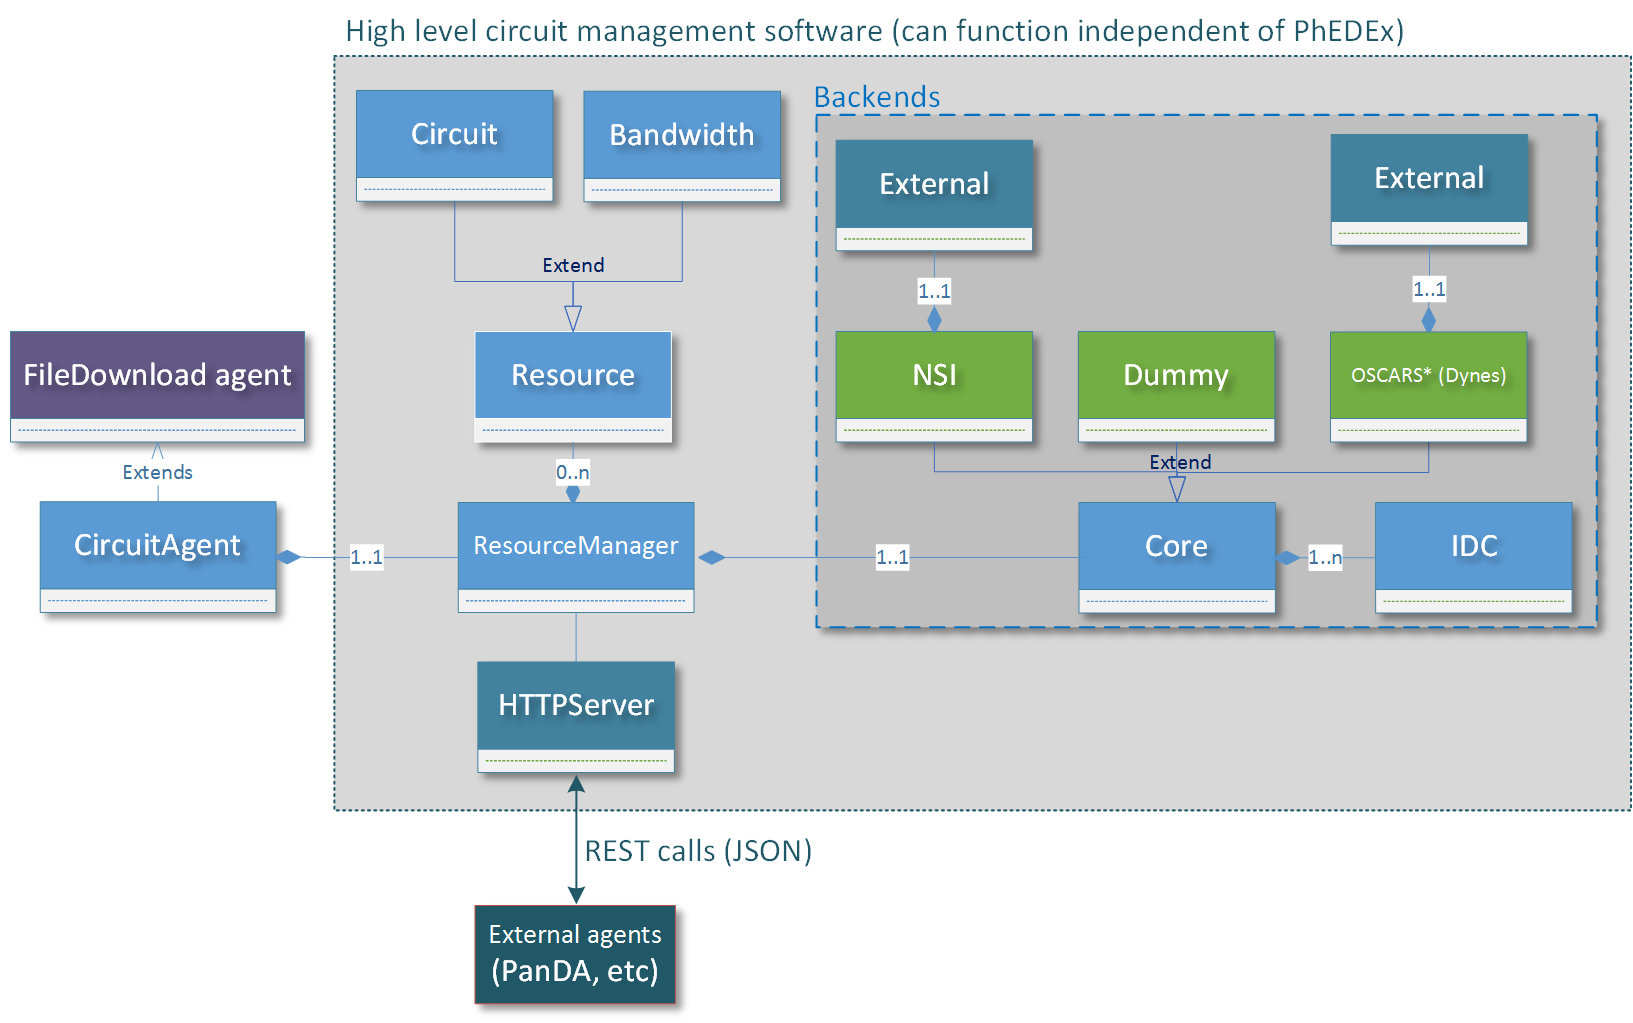
\includegraphics[width=0.95\textwidth]{Figures/Circuit_framework-class_diagram.png}
  \caption{Class diagram of the circuit management software integrated in PhEDEx}
  \label{fig:class_diagram}
\end{figure} 

\begin{figure}[h]
  \centering
  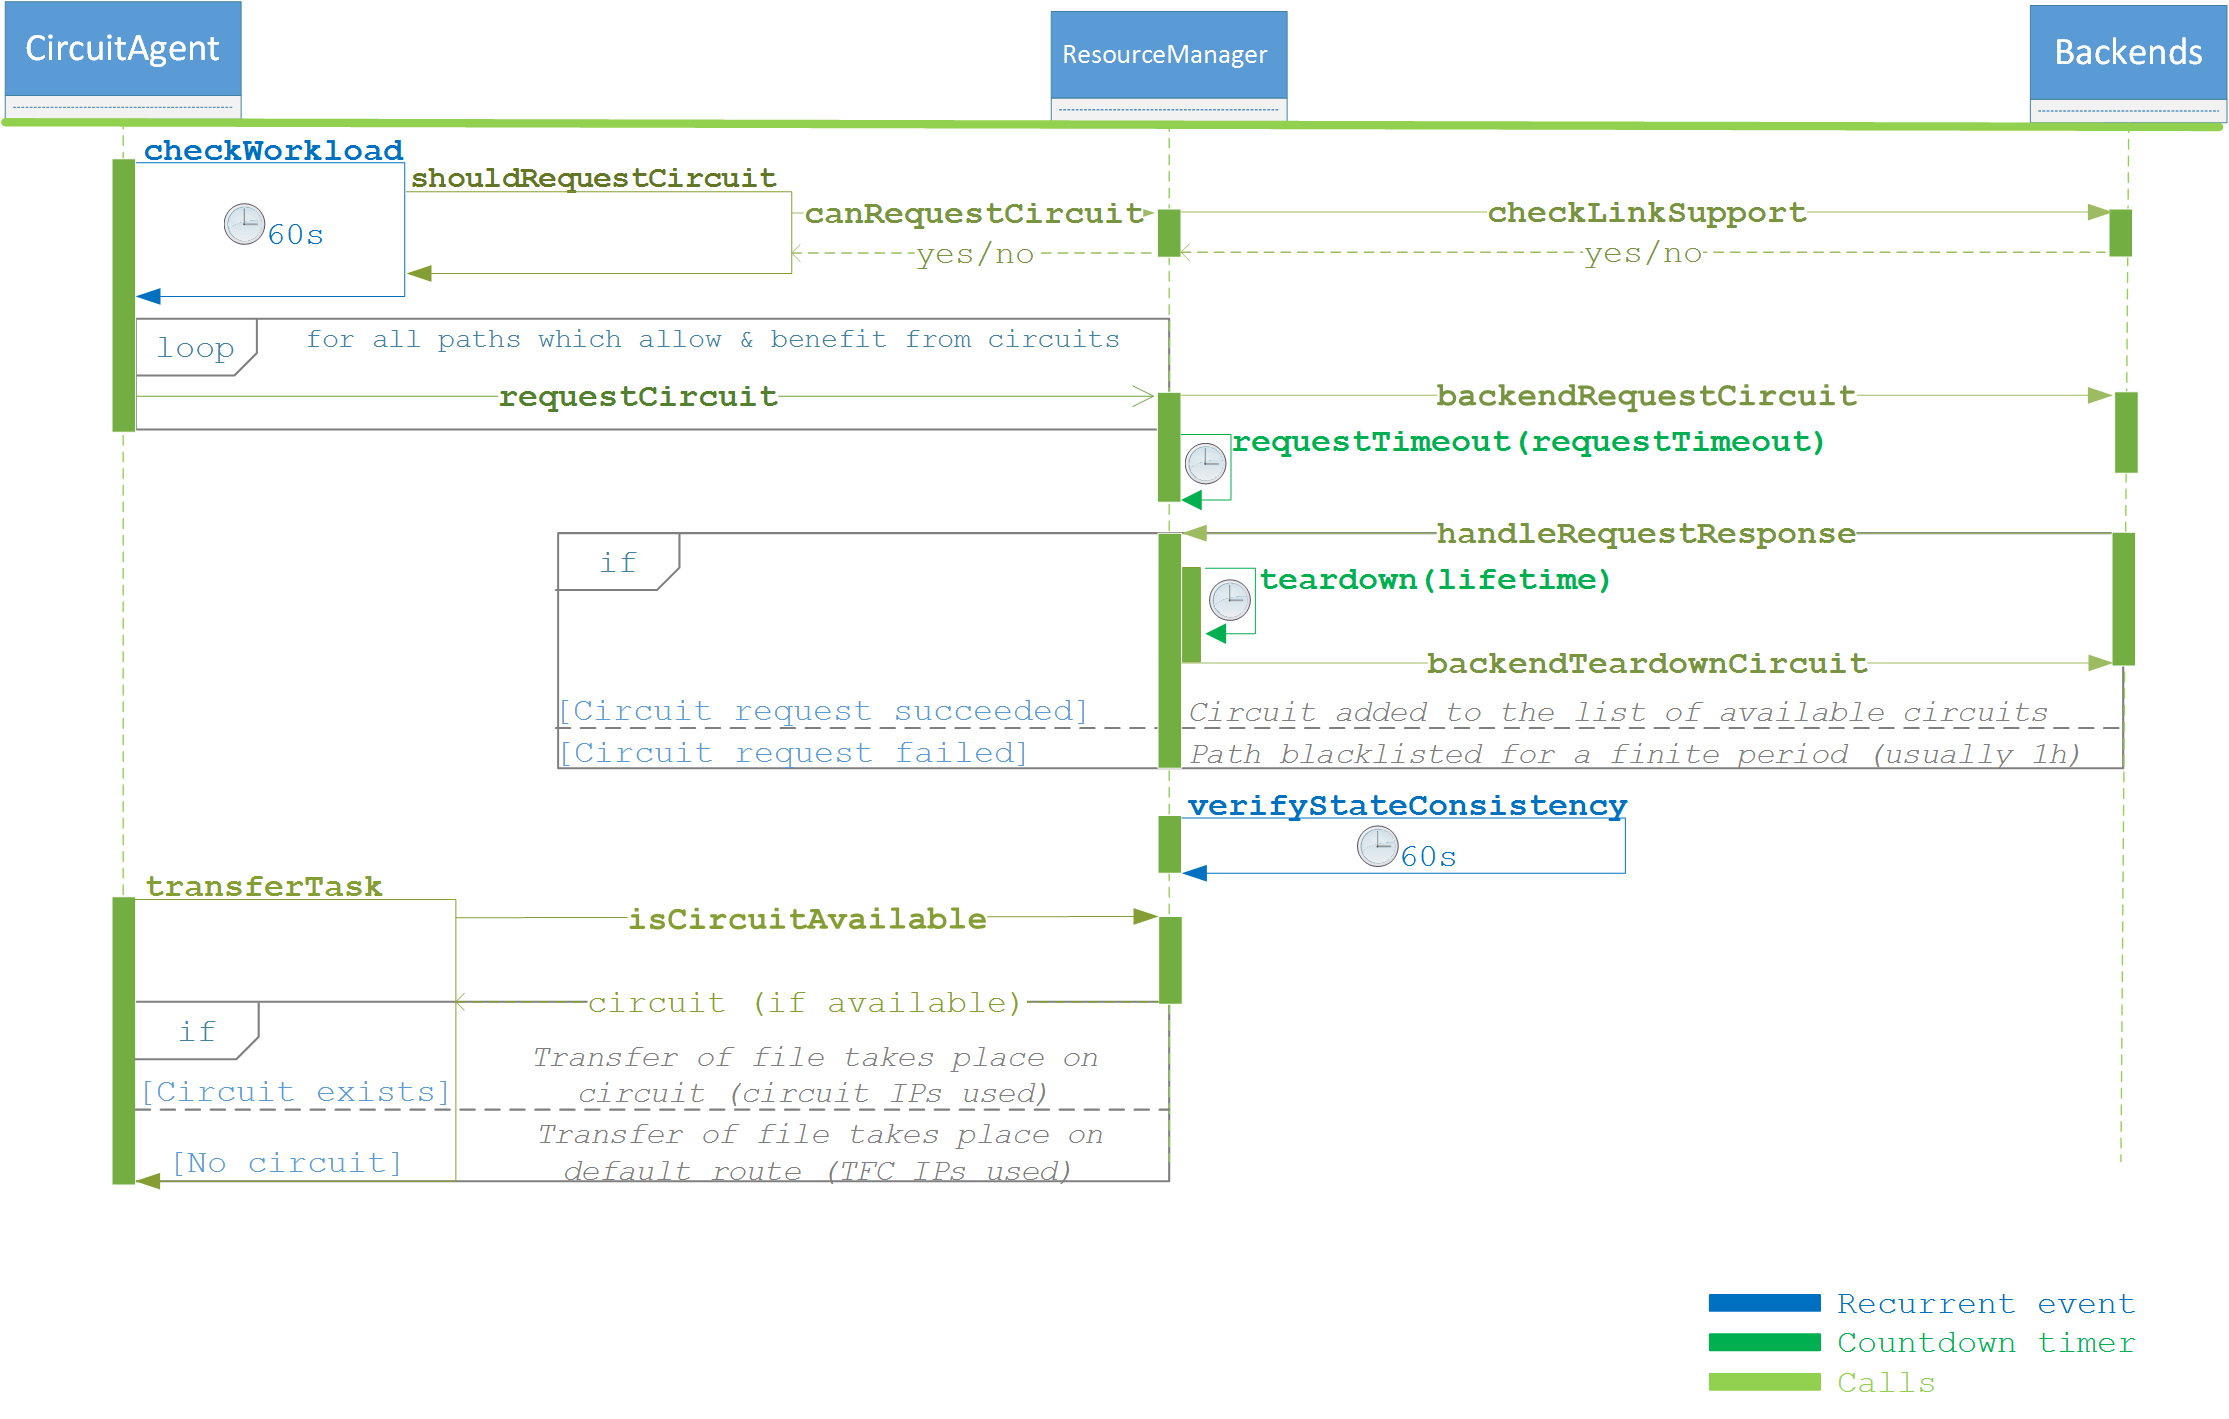
\includegraphics[width=0.95\textwidth]{Figures/Circuit_framework-sequence_diagram.png}
  \caption{Sequence diagram of the circuit management software integrated in PhEDEx}
  \label{fig:sequence_diagram}
\end{figure} 

\subsection{Circuit providers}

When ANSE began it was supposed to use the Dynes infrastructure to provide Layer 3 circuits 
between a select number of sites. Dynes was regarded as a "dynamic network cyber-instrument"
and spanned over 40 US universities and 14 Internet2 connectors. It was based on the 
implementation of Inter-Domain Circuit protocol developed by ESnet and Internet2 (with 
cooperative development from GEANT and GLIF as well).

As official funding ended for Dynes, the lack of continued support forced a switch to different 
technologies. To this end, NSI was chosen as the replacement for Dynes as it is presently 
supported by many important network providers around the globe (ESnet, Internet2, GEANT, etc.)

\subsubsection{What is NSI?}

NSI stands for Network Service Interface and is defined as the interface between a
NS requestor agent and a NS provider agent, to request a transport connection.
The requestor could be a host, middleware or network provider, while the provider 
could be a home or campus network, or even a national infrastructure provider.

NSI provides different functionalities:
\begin{itemize}
  \item Resource management: Scheduling, reservation, instantiation, negotiation
  \item Resource information: Service discovery, topology exchange, monitoring, history, security
\end{itemize}

NSI supports a tree and chain model of service chaining, and it's effectively a two 
phase reservation system (Figure \ref{fig:NSI_RSM}).

\begin{itemize}
  \item First phase
	\begin{itemize}
		\item Reservation is made
		\item Availability is checked
		\item Resources are (temporarily) held
	\end{itemize}
  \item Second phase
	\begin{itemize}
		\item Requestor commits or aborts the reservation
		\item Should the requestor fail to act within a certain time limit, the reservation is released
	\end{itemize}
\end{itemize}

\begin{figure}[h]
  \centering
  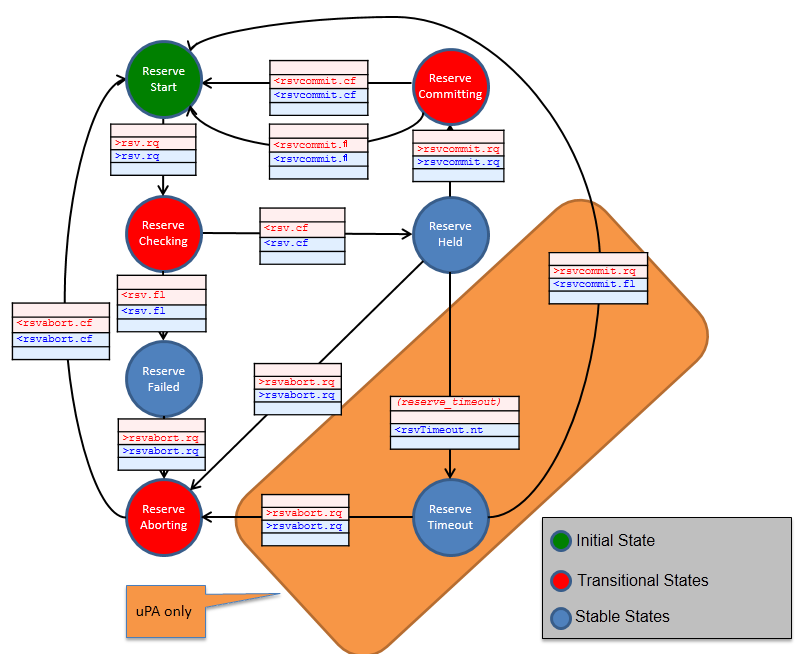
\includegraphics[width=0.95\textwidth]{Figures/NSI_RSM.png}
  \caption{The NSI Reservation State Machine}
  \label{fig:NSI_RSM}
\end{figure} 

The NSI plug-in implemented in our software uses an NSI CLI tool which was provided by ESnet.

\section{Finding a solution}

The software presented in the previous section, came a long way from the prototype 
that preceded it, however the complete solution to bringing circuit awareness and 
management into production is still under development.

\subsection{Difficulties in using NSI}

Although NSI is now the most popular implementation that promises to provide 
circuits in a production environment, it comes nonetheless with a few limitations.

\begin{description}[style=unboxed,leftmargin=0cm]
  \item[Provides a layer 2 circuit:] In contrast to Dynes which provided Layer 3 
  circuits between two servers, NSI only provides a Layer 2 circuit. This means that 
  the transfer backends used in PhEDEx cannot directly use it. A Layer 3 path 
  has to be created on top of the Layer 2 circuit. Constructing such a path means 
  having privileged access to the site's network infrastructure - something that is 
  not trivial, especially with the start of LHC operations in 2015.
  \item[Circuit ends at the border router:] The Layer 2 path doesn't end at the storage 
  servers, nor does it end at the storage farm's router. The Layer 3 path needs to 
  be created not just on top of the circuit, but also from the border routers to the 
  storage 
  \item[Guarantee bandwidth is not supported by all providers:] The motivation of using 
  circuits in PhEDEx is two fold: provide more deterministic transfer times and 
  provide a way of privileging select traffic. If even a single circuit provider 
  involved in an inter-domain transfer doesn't guarantee the bandwidth which PhEDEx 
  asks for, then the advantages of using circuits in PhEDEx may be lost.
  \item[NSI adoption is still limited:] Even though NSI has a lot more support from 
  big network providers, adoption into production is still limited at this time. 
\end{description}

\subsubsection{Difficulties in dealing with Layer2 circuits}

Since the transfer backends can't directly used Layer 2 circuits, a Layer 3 path needs to be 
established between the storage servers, or at least between the routers of the storage farms.

Establishing a Layer 3 path, is non-trivial since:
\begin{description}[style=unboxed,leftmargin=0cm]
  \item[It requires topology and routing info:] PhEDEx is a very high-level software. It only 
  knows about its transfer queue, name of sites, and name and sizes of datasets, blocks and 
  files. Its monitoring information is limited and the PFNs involved in the transfer don't 
  point directly to the file replica used in the data movement. 
  \item[Direct access to the site's network:] Perhaps the biggest challenge in establishing 
  a Layer 3 path is the fact that one requires direct access to the site's network infrastructure.
  Doing live modifications of the routing information on any production network is controversial 
  enough, even more so given that the infrastructure is critical to the success of LHC's 
  Run 2.
\end{description}

\subsection{Difficulties in using FTS/SRM}

Not all difficulties in coming up with a solution stem from using NSI as a circuit backend.
FTS/SRM and gridFTP are the most popular protocols involved in data transfer and naturally 
any solution that we propose should at the very least work with them. 

The problem here is best described in Figure \ref{fig:SURL-to-TURLs}.

In a (PhEDEx) file transfer, two PFNs are always involved: the source and destination PFNs. 
Ideally, these PFNs should directly point to the physical storage location 
of the files that need to be transferred. With FTS and SRM, the PFNs don't reflect that. 
They are only Storage URLs (SURL) and they point to the storage farm's FTS server. 
In order to get the exact location of the file, FTS needs to pick a file replica from one 
of the storage elements. Only once that's done, and the SURL is transformed into a Transfer 
URL (TURL), can a transfer begin.

This is particularly important because the actual servers involved in the transfer, 
must be known in order to establish circuits between them.

\begin{figure}[h]
  \centering
  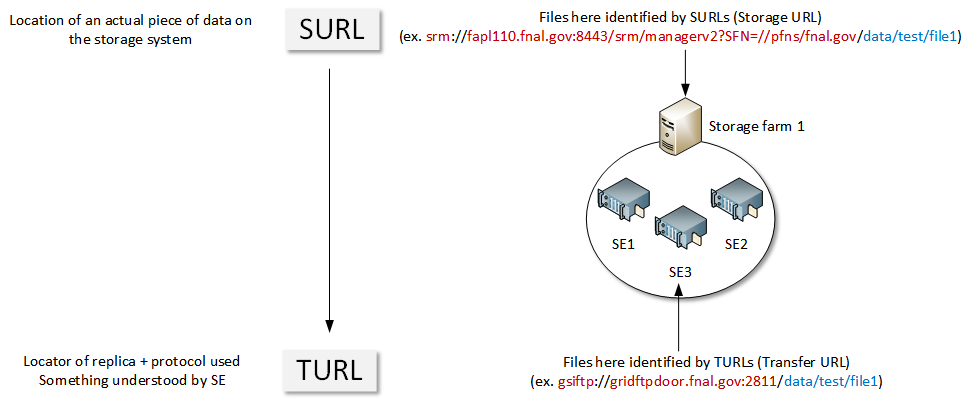
\includegraphics[width=0.95\textwidth]{Figures/TURL_to_SURL.png}
  \caption{View of PhEDEx-only transfers on both the shared and dedicated path}
  \label{fig:SURL-to-TURLs}
\end{figure} 

\subsection{Proposed solution}

Ideally, any proposed solution should:
\begin{itemize}
	\item Work in a multiple VO environment
	\item Try and deal with privileged and unprivileged traffic on the same path
	\item Work with FTS/SRM and gridFTP
	\item Be as un-intrusive into the site's operations as possible
\end{itemize}

The solution which was put forward is presented in Figures \ref{fig:global-solution-view} 
and \ref{fig:zoom-solution-view}. 

\begin{itemize}
	\item The ResourceManager is used to request a Layer 2 circuit between the border routers
	of sites A and B. The request can come from either PhEDEx or any external application that 
	uses our REST API.
	\item Once the Layer 2 circuit is up:
		\begin{itemize}
			\item A wrapper is used to retrieve all the storage servers (looking in the TURLs) 
			involved in the transfer. This information is passed to an OpenFlow controller
			\item The ResourceManager informs the OpenFlow controller that a new Layer 2 path 
			is available.
		\end{itemize}
	\item The OpenFlow controller adds routing information in all the OpenFlow switches, 
	directing all traffic coming from servers involved in the transfer, onto the newly created 
	circuit
\end{itemize}

\begin{figure}[h]
  \centering
  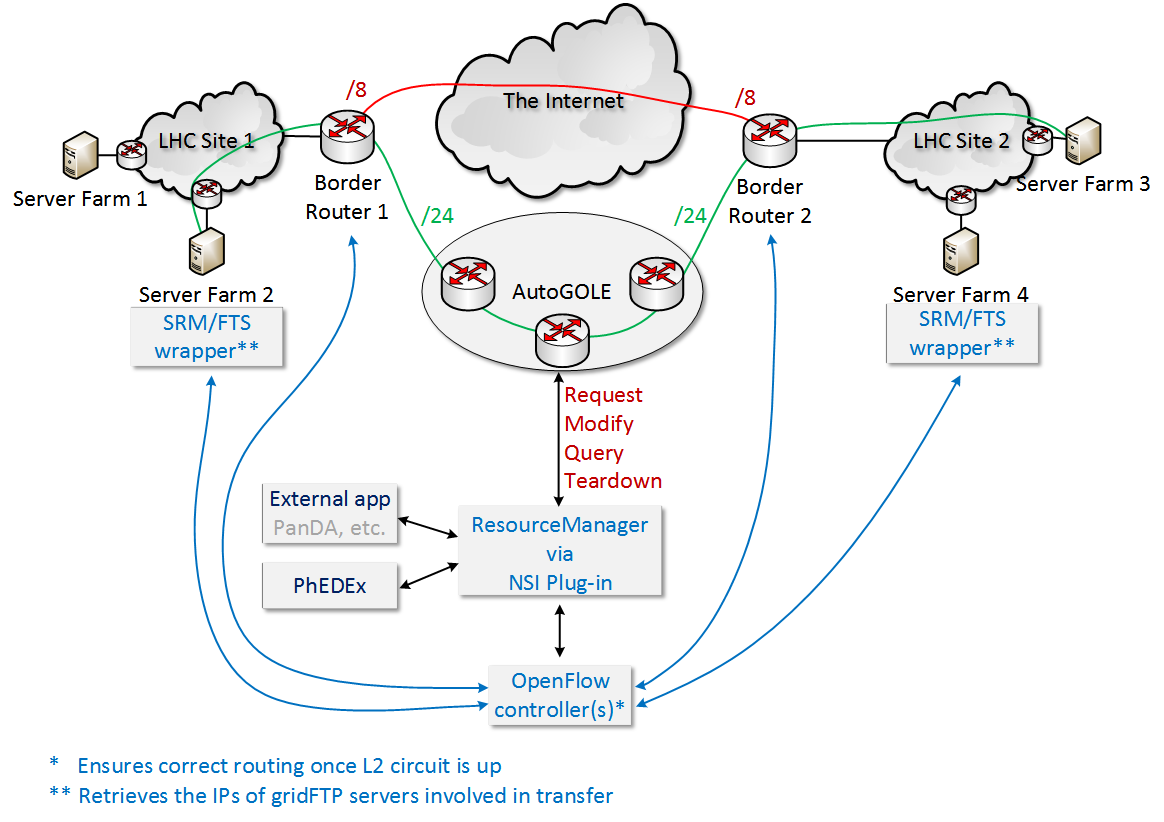
\includegraphics[width=0.95\textwidth]{Figures/Proposed_solution-global_view.png}
  \caption{Global view of our proposed solution}
  \label{fig:global-solution-view}
\end{figure} 

\begin{figure}[h]
  \centering
  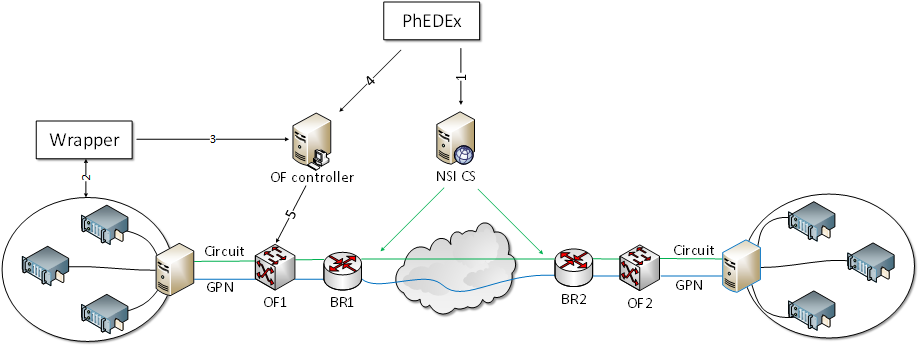
\includegraphics[width=0.95\textwidth]{Figures/Proposed_solution-zoom_view.png}
  \caption{In depth view of our proposed solution}
  \label{fig:zoom-solution-view}
\end{figure}

Some parts in this proposed architecture are still under development, specifically
the wrapper and the OpenFlow controller code, and this is where effort is 
currently being invested.
Once ready, this solution will work with the most common transfer backends in CMS,
and will be able to support traffic prioritisation in a multiple VO environment. 
Layer 3 routing will be assured by OpenFlow controllers, so there will be no need 
to resort to Policy Based Routing (PRB) and marking of privileged packets to achieve that.
By avoiding PBR and packet marking, interference with site's operations is also reduced.
\section{Summary and future plans}

PhEDEx has been very successful at managing data-flows on the WAN for the CMS 
collaboration. Nonetheless, its architecture is based on design decisions that 
start to become invalid, and in order to continue to scale and perform for the 
future, it must evolve, taking advantage of new technologies.

Over the course of the past two years, the ANSE project has made significant 
progress towards integrating network awareness into PhEDEx. A prototype was created and 
tested , demonstrating the essential features required for circuit integration 
into PhEDEx. Using the lessons learned during the prototype development, a new improved 
version was designed, which is going to be released in production shortly. 
The new system is capable of functioning independently from PhEDEx, it can be 
controlled remotely via a REST interface and it is modular, being able to use 
multiple circuit providers.

The remaining work in ANSE, focuses more on the network aspect of the solution.
While the PhEDEx software is ready to make use of circuits as soon as they mature 
into a production ready version, the interim solution still relies on more work 
on our part, mainly in extending a circuit from storage to storage. 
This is where ANSE will invest its resources in the following months.
\begin{thebibliography}{1}

\bibitem{PhEDEx}
 Egeland R, Metson S and Wildish T 2008 Data transfer infrastructure for CMS data taking,  {\it XII Advanced Computing and Analysis Techniques in Physics Research (Erice, Italy: Proceedings of Science)}

\bibitem{CMS}
 The CMS Collaboration 2008 The CMS experiment at the CERN LHC {\it JINST {\bf 3} S08004}

\bibitem{WLCG}
 Eck C {\it et al.} 2005 LHC Computing Grid Technical Design Report {\it CERN-LHCC-2005-024}

\bibitem{TW_DB_CHEP13}
 Bonacorsi D and Wildish T 2013 Challenging CMS Computing with Network-Aware Systems {\it submitted to CHEP 2013}
 
\bibitem{ANSE}
 LHCONE Point-to-Point Service Workshop, December 2012 
 {\it http://indico.cern.ch/event/215393/session/1/contribution/8/material/slides/1.pdf}
 
\bibitem{ANSE-ISGC}
International Symposium on Grids and Clouds 2014 {\it http://pos.sissa.it/archive/conferences/210/021/ISGC2014\_021.pdf}

\bibitem{FDT}
 Fast Data Transfer (FDT) {\it http://fdt.cern.ch/}

\bibitem{IDCP}
 InterDomain Controller Protocol {\it http://www.controlplane.net/}

\bibitem{OSCARS}
  Guok C, Robertson D, Thompson M, Lee J, Tierney B, Johnston W 2006: Intra and Interdomain Circuit Provisioning Using the OSCARS Reservation System {\it ICBCNS 2006}

\bibitem{FTS}
 Alvarez Ayllon A, Kamil Simon M, Keeble O and Salichos M 2013 FTS3 - Robust, simplified and high-performance data movement service for WLCG {\it submitted to CHEP 2013}

\bibitem{DYNES}
 Dynes: DYnamic NEtwork System {\it https://www.terena.org/activities/e2e/ws3/slides/101129-dynes-Artur.pdf}

\bibitem{PANDA}
  ATLAS collaboration, 2008: PanDA: distributed production and distributed analysis system for ATLAS {\it Journal of Physics: Conference Series, Volume 119, Part 6}
 
\bibitem{NSI}
 OGF Network Service Interface {\it https://www.terena.org/activities/e2e/ws2/slides2/11\_NSI\_Eduard.pdf}

\bibitem{NSI-CS2}
 NSI Connection Service v2 {\it https://www.ogf.org/documents/GFD.212.pdf}

\end{thebibliography}


\end{document}